\subsubsection{GemNet}
\label{subsubsec:gemnet}

Gasteiger et al. proposed GemNet \cite{https://doi.org/10.48550/arxiv.2106.08903} 
as an improvement over DimeNet and DimeNet++ (see 
\cite{DBLP:journals/corr/abs-2003-03123, https://doi.org/10.48550/arxiv.2011.14115} 
and \ref{subsubsec:dimenet}) in which essentially also quadruplets of nodes are
taken into account. 

Just like DimeNet and DimeNet++, GemNet (\enquote{Geometric Message Passing Neural Network}) takes the positions $\XX$ and atomic numbers 
$\zz$ of a molecule (defined in \eqref{eq:molecule_setup}) as inputs. For
$a, b \in \set{1, \dots, n}$ write
\[
    x_{ab} \: \coloneqq \: \norm{\xx_a - \xx_b}_2 
    \qquad \text{and} \qquad 
    \vec{\xx}_{ab} \: \coloneqq \xx_b - \xx_a
\]
for the distance and relative direction from $\xx_a$ to $\xx_b$ respectively.
\begin{wrapfigure}{r}{0.3\textwidth}
    \centering
    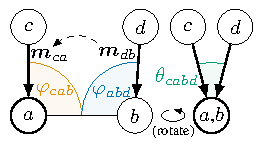
\includegraphics[]{atomic_simulations/gemnet_message_passing.pdf}
\end{wrapfigure}
In GemNet, there are two graphs considered: an interaction graph and an embedding graph.
The molecule's interaction graph does not change during the forward pass of the network and 
two atoms \textit{interact} if their distance is below some 
cutoff $c_{\text{int}}$. In addition to this interaction graph, all atom pairs 
whose distance is below some threshold $c_{\text{emb}}$ are \textit{embedded}---and, thus, edges 
of the embedding graph.

In contrast to DimeNet, quadruplets of 
nodes are now taken into account for message passing: Consider pairwise different $a, b, c, d \in \set{1, \dots, n}$,
where $(x_{ab}, a, b)$ are interacting and $(\_, c, a)$, $(\_, d, b)$ are
embedded. Set
\[
    \varphi_{cab} \: \coloneqq \: 
    \measuredangle \left( \vec{\xx}_{ca}, \vec{\xx}_{ab} \right)
    \qquad \text{and} \qquad
    \varphi_{abd} \: \coloneqq \: 
    \measuredangle \left( \vec{\xx}_{ab}, \vec{\xx}_{db} \right) \text{,}
\]
as well as 
\[
    \phi_{cabd} \: \coloneqq \: \measuredangle \left( \boldsymbol{\Pi} \vec{\xx}_{ca}, \boldsymbol{\Pi} \vec{\xx}_{db} \right),
    \qquad \boldsymbol{\Pi} \: \coloneqq \: \boldsymbol{I}_3 - \vec{\xx}_{ab} \vec{\xx}_{ab}^\top \text{,}
\]
where $\boldsymbol{\Pi}$ is the orthogonal projection onto the orthogonal
complement of $\vec{\xx}_{ab}$.

Similarly to DimeNet, this relative directional information is then represented 
by spherical Fourier-Bessel bases
\[
    \eee_{\text{RBF}}^{(ca)} \: = \: \eee_{\text{RBF}}(x_{ca}), 
    \quad \eee_{\text{CBF}}^{(cab)} \: = \: \eee_{\text{CBF}}(x_{ca}, \varphi_{cab}),
    \quad \eee_{\text{SBF}}^{(cabd)} \: = \: \eee_{\text{SBF}}(x_{ca}, \varphi_{cab}, \phi_{cabd}) 
    \text{.}
\]
After this setup phase, initial node embeddings $\hh_{a}^{(1)}$, edge embeddings 
$\mm_{ca}^{(1)}$ (for each pair $(c, a)$ of nodes that is embedded) and outputs
$t_{a}^{(1)}$ or a global attribute $t^{(1)} = \sum_{a=1}^n t_a^{(1)}$
are computed based on $\zz$ and $\eee_{\text{RBF}}^{(ca)}$. 

The initial input graph can now also be roughly expressed in the
EGN framework (see \ref{subsubsec:egns} and 
\cite{https://doi.org/10.48550/arxiv.2203.09697}) as follows:
\[
    G \: = \: (t^{(1)}, V^{(1)}, E^{(1)}, T^{(1)})
\]
with nodes and edges
\begin{align*}
    V^{(1)} \: &\coloneqq \: \setcomp{\hh_{a}^{(1)}}{a \in \set{1, \dots, n}}, \\
    E^{(1)} \: &\coloneqq \: \setcomp{(\mm_{ca}^{(1)}, c, a)}{c, a \in \set{1, \dots, n}, \: x_{ca} \leq c_{\text{emb}}}
\end{align*}
as well as 3- and 4-way interactions
\begin{align*}
    T^{(1)} \: &\coloneqq \quad \setcomp{(\_, c, a, b)}{c, a, b \in \set{1, \dots, n}, \: x_{ca} \leq c_{\text{emb}}, \: x_{ab} \leq c_{\text{int}}} \\
    &\qquad \cup  \setcomp{(\_, c, a, b, d)}{c, a, b, d \in \set{1, \dots, n}, \: x_{ca} \leq c_{\text{emb}}, \: x_{ab} \leq c_{\text{int}}, \: x_{db} \leq c_{\text{emb}}};
\end{align*}
where the higher-order attributes are handled implicitly (denoted by \enquote{$\_$}) 
based on the node and edge embeddings, are indexed by the involved nodes (contrary to \eqref{eq:higher_order_interact}),
 and all appearing $a, b, c, d$ are assumed to be 
pairwise different.

This input graph is now successively updated in the GN/EGN scheme using a sequence of complex interaction
blocks in which the relative directional information 
$\eee_{\text{RBF}}^{(ca)}$, $\eee_{\text{CBF}}^{(cab)}$, $\eee_{\text{SBF}}^{(cabd)}$ is put to use. 
The complete GemNet architecture as depicted in 
\cite{https://doi.org/10.48550/arxiv.2106.08903} can be seen in Figure~\ref{fig:gemnet}.

\begin{figure}[H]
    \centering
    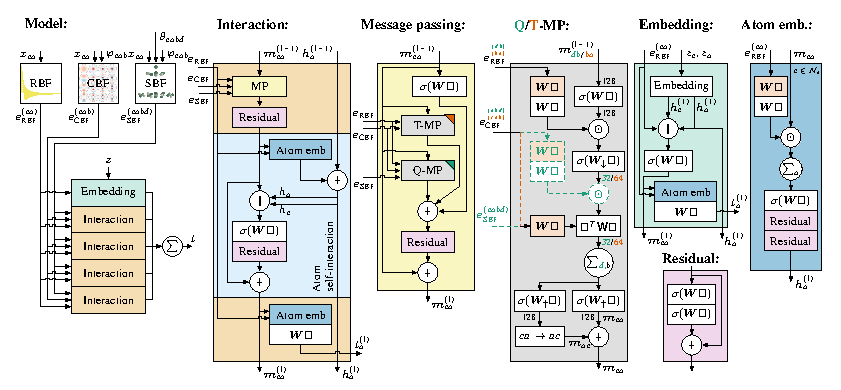
\includegraphics[]{atomic_simulations/gemnet.pdf}
    \caption{Complete architecture of GemNet as depicted in \cite[Appendix F]{https://doi.org/10.48550/arxiv.2106.08903}.}
    \label{fig:gemnet}
\end{figure}
